\documentclass[red]{beamer}

\usepackage[italian]{babel}
\usepackage[utf8]{inputenc}
\usepackage{pgf}
\usepackage{wrapfig}

\graphicspath{{./img/}}

\newtheorem{defs}{Definizione}[section]

\mode<presentation>{
    \usetheme[left]{Marburg}
    \useinnertheme[shadow]{rounded}
}

\AtBeginSubsection[]
{
  \begin{frame}<beamer>{Contenuti}
    \tableofcontents[currentsection,currentsubsection]
  \end{frame}
}

\title[Software per segnali radioastronomici]{Sviluppo di un software per l'analisi real-time di dati
radioastronomici su macchine multicore}
\author{Stéphane Bisinger}


\begin{document}

\begin{frame}
	\titlepage
\end{frame}

\begin{frame}{Riassunto}
	\tableofcontents
\end{frame}

\section{Teoria}
\subsection{Analisi dei segnali}
\begin{frame}{Cosa sono e come si analizzano i segnali?}
	\transdissolve<2>
	\begin{defs} \label{def:signal}
		Si dice segnale una qualunque quantità che varia nel tempo o nello spazio.
	\end{defs}

	\only<1>{Ad esempio un suono è un segnale frutto della variazione di
	pressione dell'aria nel tempo.}
	\only<2>{Un segnale può essere rappresentato in funzione delle frequenze
	delle sinusoidi che lo compongono.}
	\begin{center}
		\only<1>{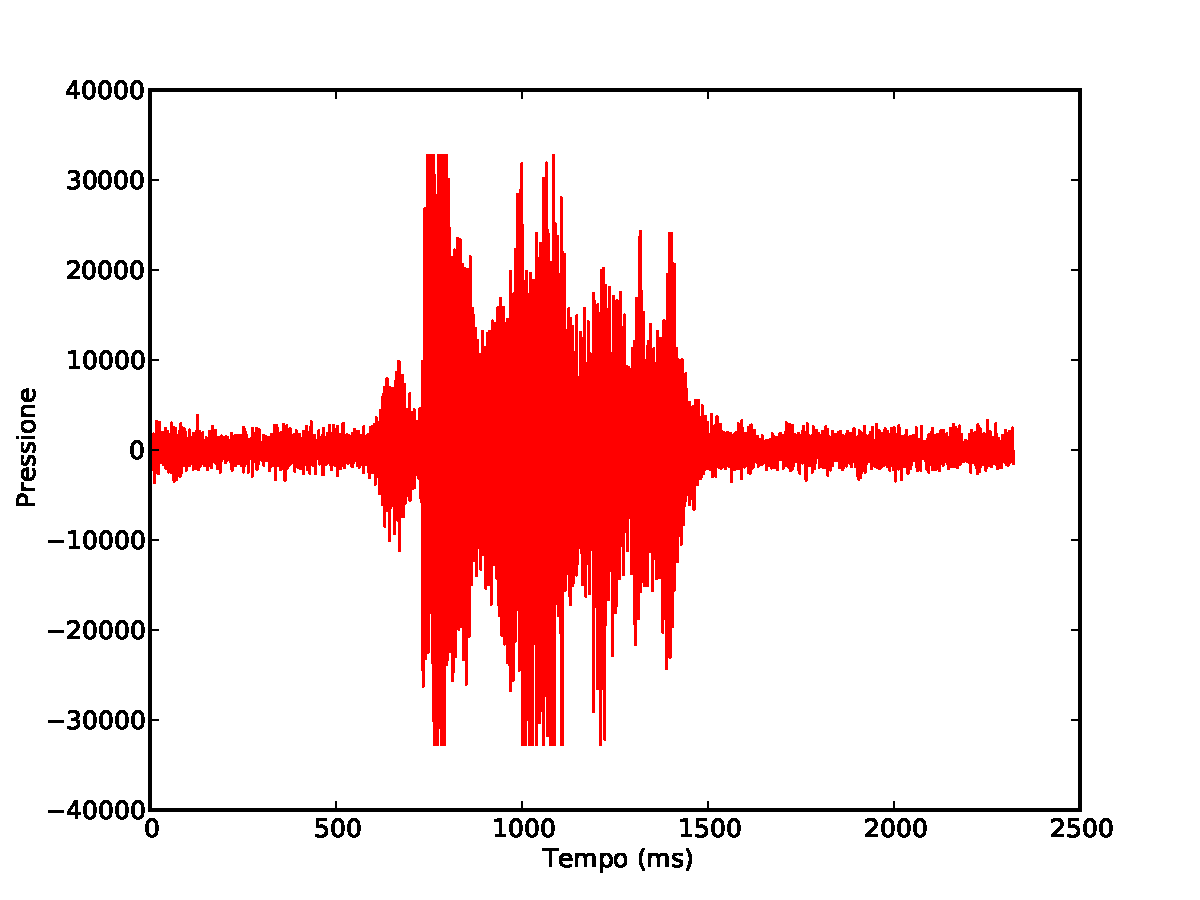
\includegraphics[width=0.7\textwidth]{segnale}}
		\only<2>{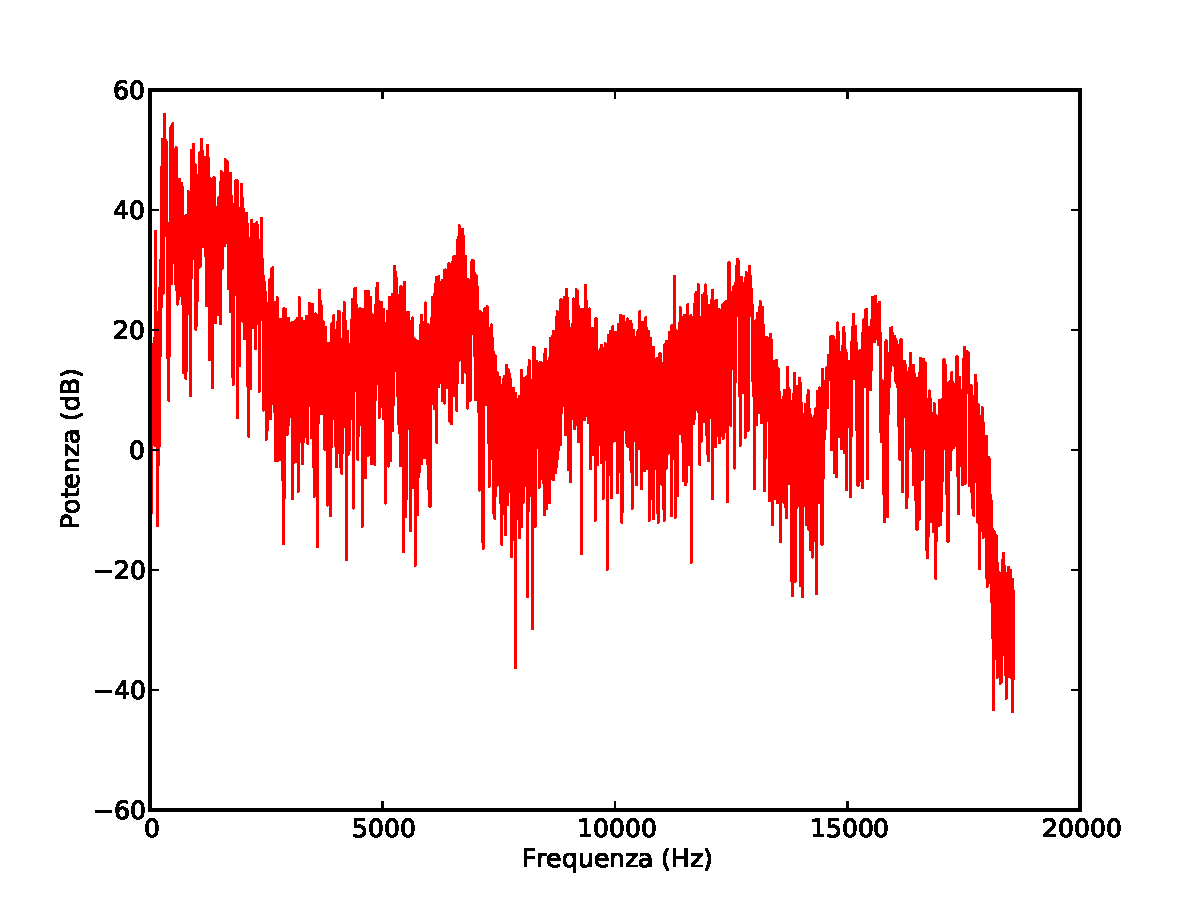
\includegraphics[width=0.7\textwidth]{frequenza}}
	\end{center}
\end{frame}

\subsection{Radioastronomia}
\begin{frame}{I radiotelescopi}
	Un radiotelescopio osserva le onde elettromagnetiche provenienti dallo spazio
	con frequenze comprese tra i 70 Mhz ed i 43 Ghz, dette onde
	\emph{radio}.
	\begin{center}
		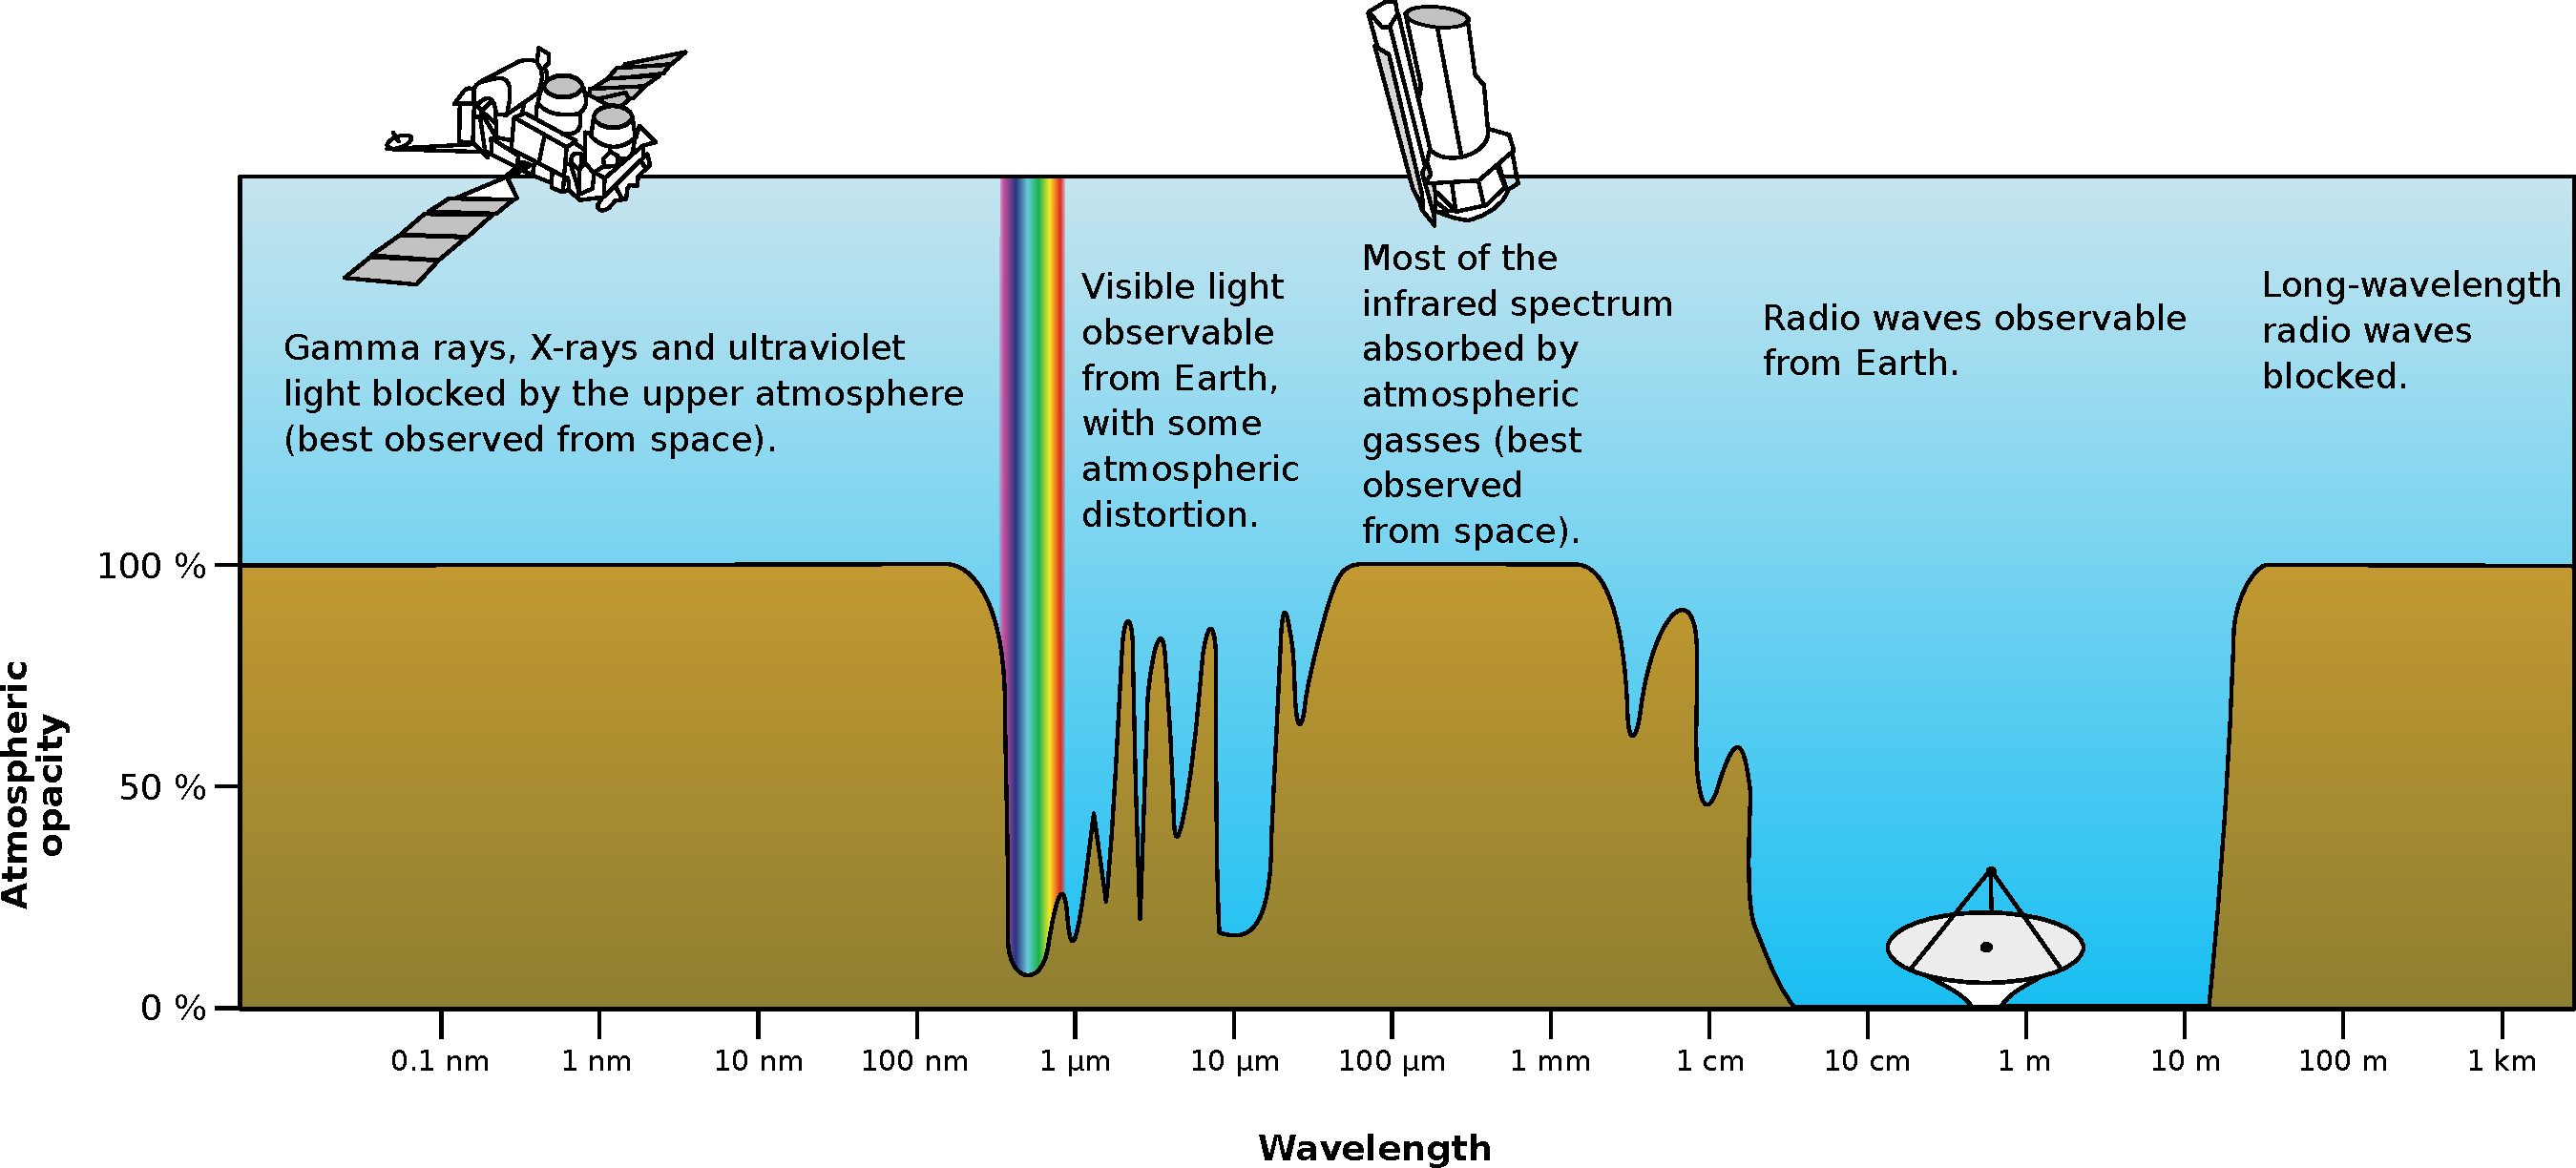
\includegraphics[width=0.7\textwidth]{Atmospheric_electromagnetic_opacity}
	\end{center}
	Le altre onde elettromagnetiche vengono in gran parte assorbite dall'atmosfera
	terrestre.
\end{frame}

\begin{frame}{I radiotelescopi di Medicina}
	\transdissolve<2-3>
	\pgfputat{\pgfxy(5.5,0)}{\pgfbox[left, base]{
\includegraphics[height=1.3cm]{logo_inaf}}}
	\begin{wrapfigure}{r}{0.5\textwidth}
		\only<1>{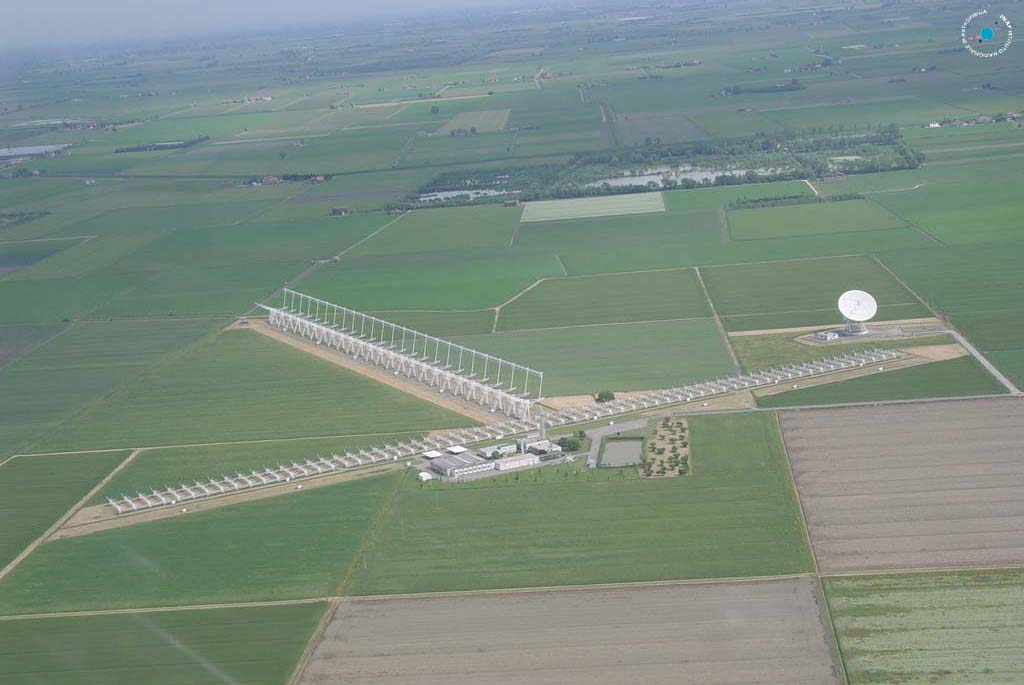
\includegraphics[width=0.45\textwidth ]{stazione1}
		}\only<2>{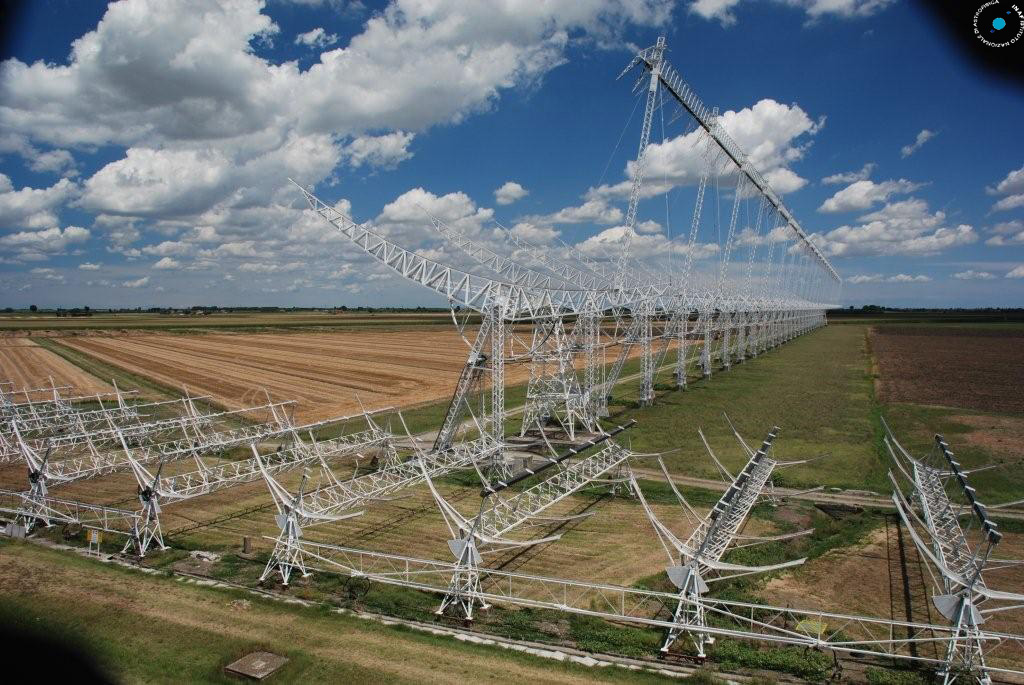
\includegraphics[width=0.45\textwidth ]{croce_del_nord}
		}\only<3>{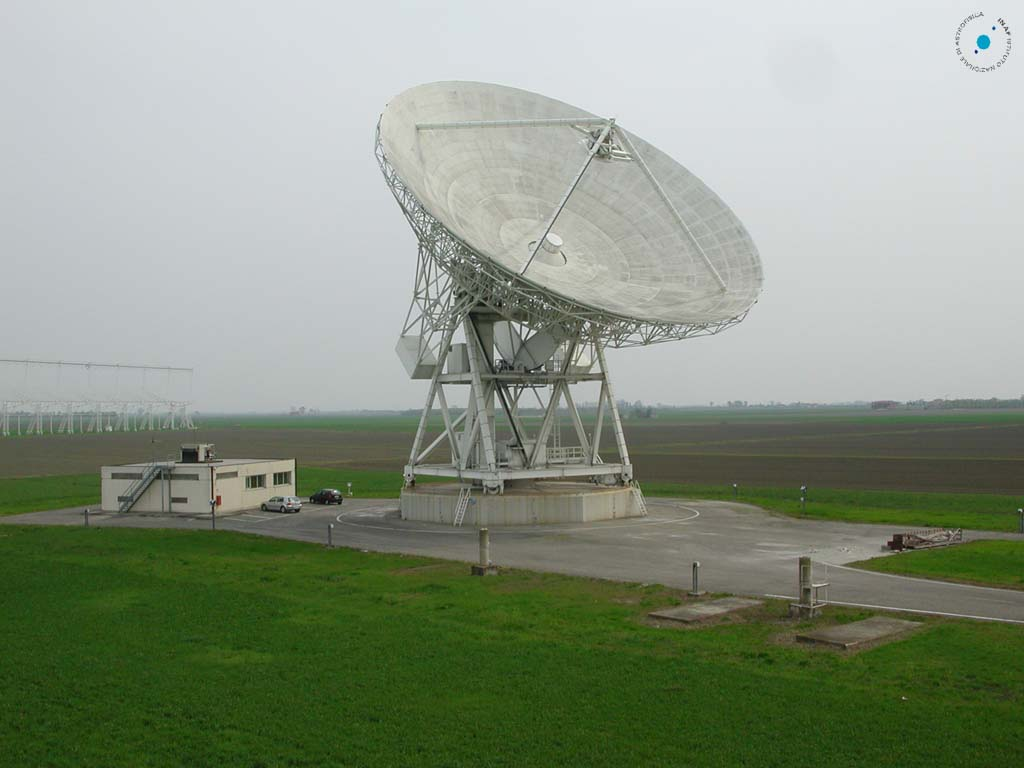
\includegraphics[width=0.45\textwidth ]{parabolica} }
		\label{fig:rtscopes}
	\end{wrapfigure}
			Inaugurata nel 1964, la stazione ``Croce del Nord'' di Medicina (BO)
			ha sancito l'inizio dell'osservazione radioastronomica in Italia,
			con la costruzione del primo radiotelescopio.

			La stazione è attualmente munita di due diversi radiotelescopi:
			\pause
			\begin{itemize}[<+->]
				\item La \alert{Croce del Nord}, costituita da due bracci,
					Nord-Sud ed Est-Ovest, per un'area collettrice di 30000
					$m^2$ totali.
				\item L'\alert{Antenna Parabolica}, con un diametro di 32 m,
					operabile sia in modalità \emph{single dish} che in rete con
					altre antenne. Partecipa al progetto \emph{VLBI}.
			\end{itemize}

\end{frame}

\section{Il software}
\subsection{Modularità}
\begin{frame}{Classi astratte}
	\begin{center}
		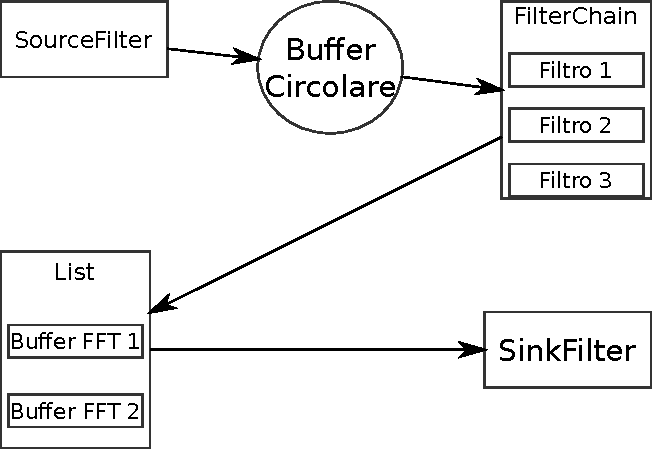
\includegraphics[width=0.4\textwidth]{algorithm}
	\end{center}
	Per rendere il software modulabile, sono state impiegate le classi
	\emph{astratte}. Grazie all'utilizzo delle classi astratte si possono
	sostituire diversi componenti con facilità:\pause
	\begin{itemize}[<+->]
		\item La \alert{fonte} da cui leggere i dati.
		\item La \alert{destinazione} verso cui inviare i dati elaborati.
		\item Le \alert{trasformazioni} da effettuare sui segnali.
	\end{itemize}
\end{frame}
\subsection{Concorrenza}
\begin{frame}{Thread principali}
	\begin{center}
		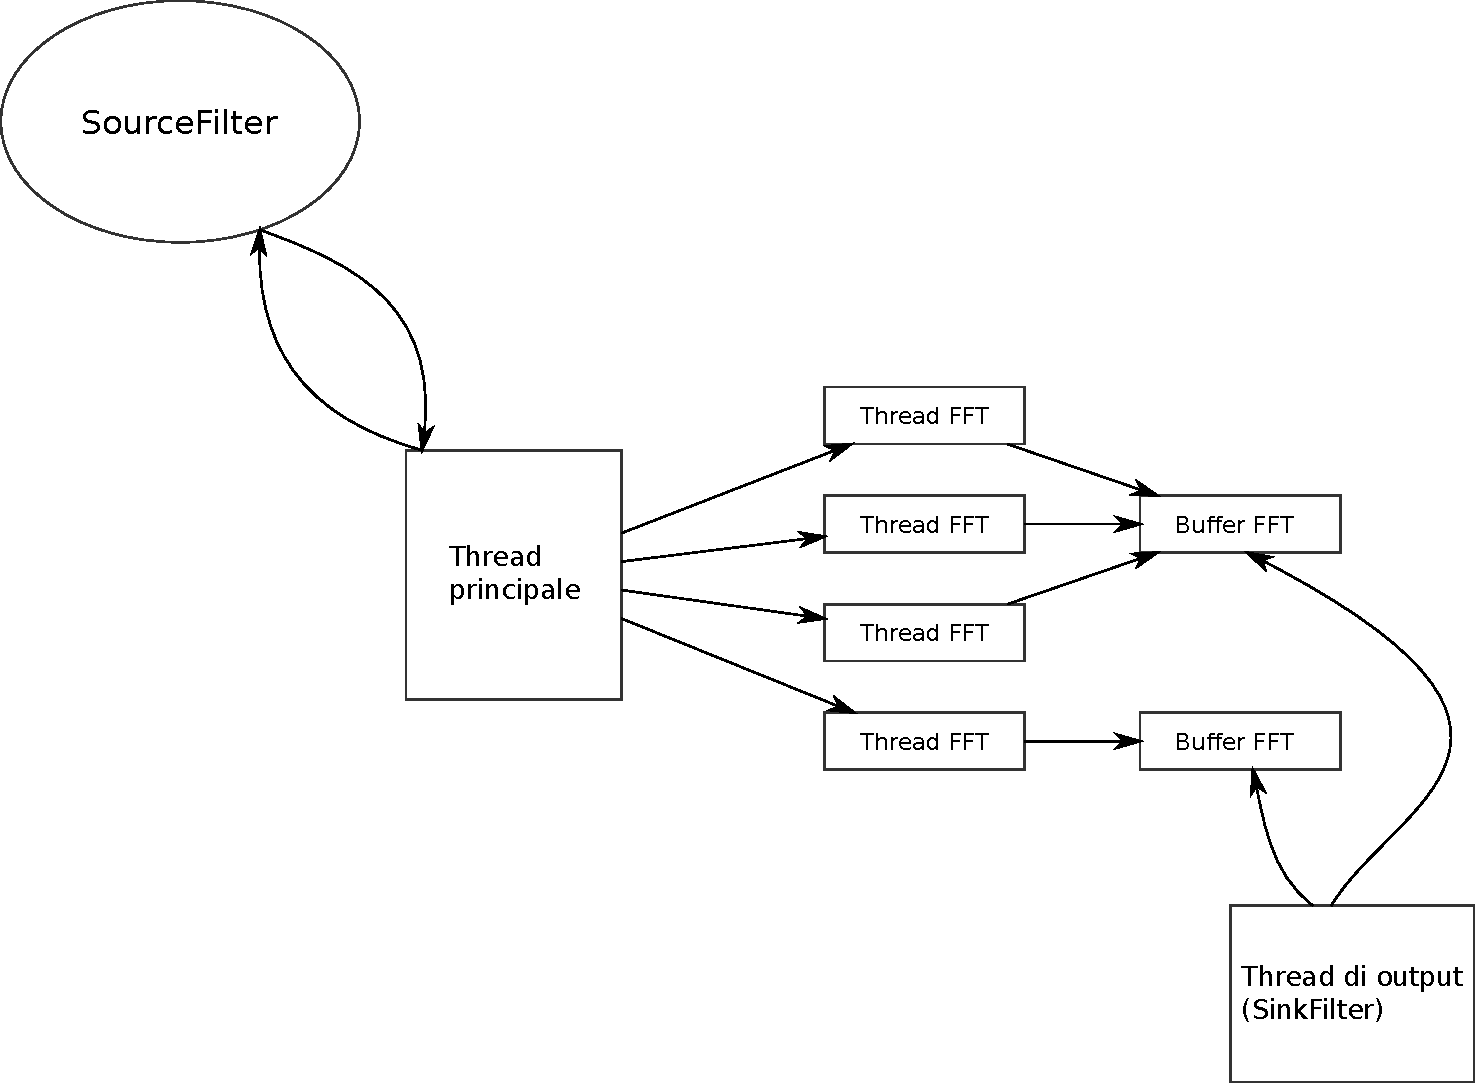
\includegraphics[height=2.7cm]{threading}
	\end{center}
	L'applicazione avvia diversi thread per sfruttare al meglio le possibilità
	offerte da processori multi-core e processori multipli. In
	particolare:\pause
	\begin{itemize}[<+->]
		\item Il \alert{thread principale}, che si occupa di avviare gli altri
			thread e di assegnare i dati ai vari thread.
		\item Un \alert{threadpool} contenente i diversi thread di lavoro, che
			si occupano di effettuare le trasformazioni.
		\item Il thread di \alert{output}, che si occupa di scrivere i dati
			elaborati sulla destinazione prescelta.
	\end{itemize}
\end{frame}
\section{Risultati e Conclusioni}
\subsection{Risultati}
\begin{frame}{Test effettuati}
	Una volta terminato lo sviluppo, si entra nella fase di testing per
	verificare il lavoro svolto. In particolare viene verificata la
	\alert{correttezza} del software, applicando le trasformazioni ad un segnale
	di cui si conosce la forma.
	\begin{center}
		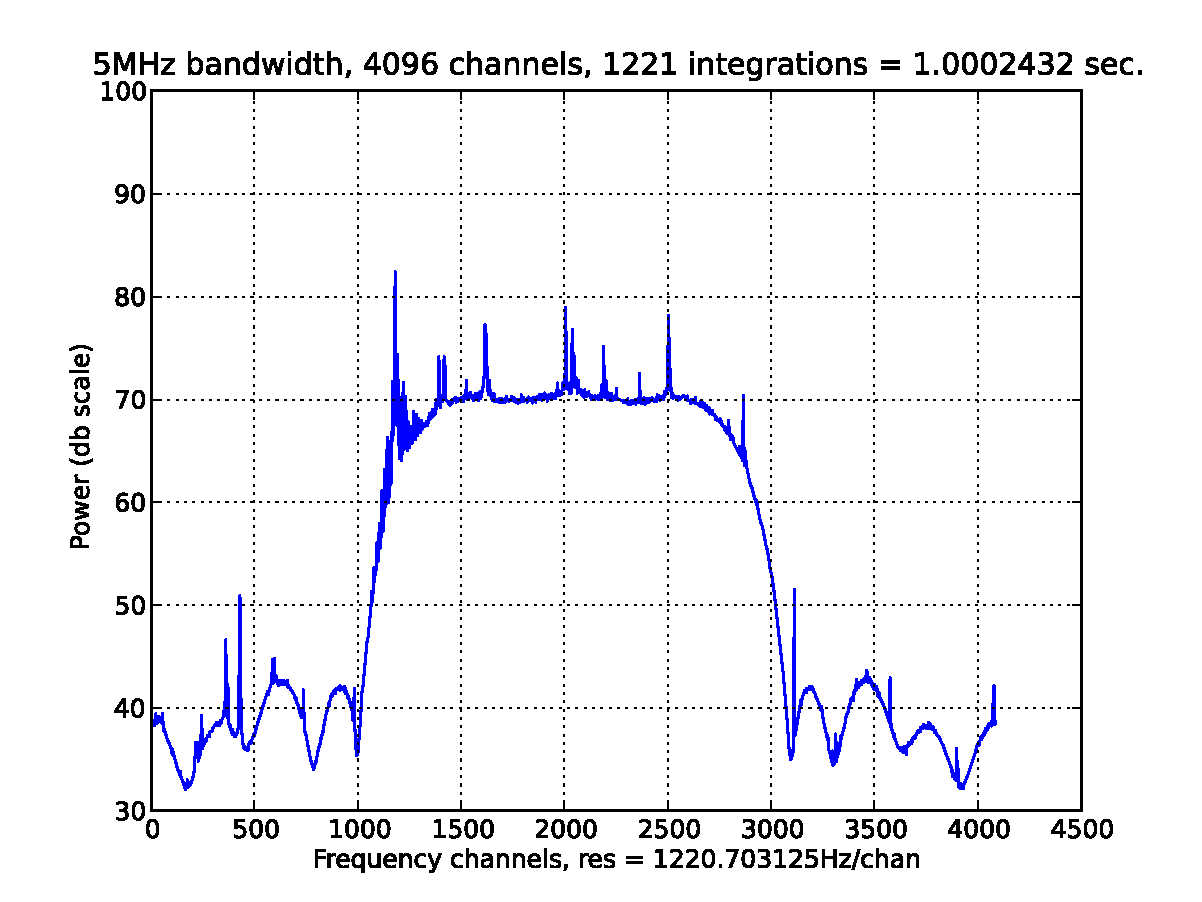
\includegraphics[width=0.65\textwidth]{5_4096_1221}
	\end{center}\pause
	In seguito si effettuano dei test atti a verificare le \alert{prestazioni}
	del software.
\end{frame}
\begin{frame}{Risultati dei test}
	\begin{tabular}{crrrl}
Can. & Integr. & T. totale & Seg. output & Tempo trasf.
\\\hline
256 & 1 & 4.831 & 94164 & 5.13041e-05\\
256 & 20 & 5.984 & 5834 & 0.00102571\\
256 & 195 & 3.952 & 394 & 0.0100305\\
256 & 195313 & 24.182 & 2 & 12.091\\
512 & 1 & 5.087 & 49583 & 0.000102596\\
512 & 98 & 9.040 & 899 & 0.0100556\\
4194304 & 1 & 6.242 & 6 & 1.04033\\
4194304 & 12 & 38.022 & 3 & 12.674\\
\end{tabular}
\end{frame}
\subsection{Conclusioni}
\begin{frame}{Conclusioni}
	Le prestazioni ottenute mostrano come la soluzione software sia
	sufficientemente matura per poter essere usata in concomitanza, o in
	sostituzione, a \emph{DSP} ed \emph{FPGA}.

	\vspace{1cm}
	Questo porta diversi vantaggi, tra cui:
	\begin{itemize}
		\item Maggior flessibilità del programma.
		\item Ottimizzazione di risorse già esistenti.
		\item Rapidità dello sviluppo.
	\end{itemize}
\end{frame}
\subsection{Sviluppi futuri}
\begin{frame}{Sviluppi futuri}
	Lo sviluppo di questo software apre la strada per tantissimi possibili
	sviluppi futuri:
	\vspace{1cm}
	\begin{itemize}[<+->]
		\item Estensione delle funzionalità del programma.
		\item Confronto con librerie alternative.
		\item Usare la scheda grafica per effettuare trasformate FFT.
		\item Ottimizzazioni e confronto tra compilatori.
			\begin{itemize}[<+->]
				\item GNU g++
				\item ICC
				\item CLang/LLVM
			\end{itemize}
	\end{itemize}
\end{frame}
\begin{frame}{\ldots so long, and thanks for all the fish!}
	Grazie dell'attenzione!
\end{frame}
\end{document}
